% === C08 - Scheduler de tareas ===
% David Alejandro Gonzalez Marquez
% dmarquez@dc.uba.ar / fokerman@gmail.com
% https://github.com/fokerman/Orga2Course

\documentclass[aspectratio=169]{beamer}
% \documentclass[handout]{beamer}

% % % Packages
\usepackage[sfdefault]{AlegreyaSans}
\usepackage{inconsolata}
\usepackage{multicol}
\usepackage{multirow}
\usepackage[spanish]{babel}
\usepackage[utf8]{inputenc}
\usepackage{enumerate}
\usepackage{color}
\usepackage{xcolor}
\usepackage[absolute,overlay]{textpos}
  \setlength{\TPHorizModule}{1mm}
  \setlength{\TPVertModule}{1mm}
\usepackage{framed}
\usepackage{mfirstuc} % para poner en mayusculas la primer letra
\usepackage{xspace} % para crear espacios en comandos 
\usepackage{pbox}
\usepackage{tikz}
\usepackage{mathabx}

% % % Beamer config
\usetheme{Pittsburgh}
\usecolortheme[rgb={1,0.48,0.0}]{structure}
\setbeamercolor{block title}{fg=white,bg=verdeuca}
\xdefinecolor{verdeuca}{rgb}{0.0,0.48,0.54}
\xdefinecolor{naranjauca}{rgb}{1,0.48,0.0}
\setbeamercolor{palette quaternary}{fg=white,bg=verdeuca}
\setbeamertemplate{title page}[default][colsep=-4bp, rounded=true] % remove title shadow
\setbeamertemplate{frametitle}[default][colsep=-2bp, shadow=false] % remove frame title shadow
\setbeamertemplate{navigation symbols}{} % remove navigation symbols
\beamertemplatenavigationsymbolsempty

% % % Colors
\definecolor{AzulClaro}{rgb}{.31,.506,.741}
\definecolor{Gris}{gray}{0.8}
\definecolor{Celeste}{rgb}{.255,.41,.884}
\definecolor{Rojo}{rgb}{1, 0, 0}
\definecolor{a}{rgb}{0.0, 0.53, 0.74}
\definecolor{r}{rgb}{0.89, 0.0, 0.13}
\definecolor{v}{rgb}{0.0, 0.5, 0.0}
\definecolor{y}{rgb}{0.0, 0.5, 0.5}
\definecolor{rojo}{HTML}{F1521B}
\definecolor{verde}{HTML}{80CD29}
\definecolor{amarillo}{HTML}{FABC09}
\definecolor{azul}{HTML}{00ADF1}

% % % Rename
\newcommand{\tab}[0]{\hspace{15pt}}

% % % Blocks
\setbeamercolor{block body}{fg=black, bg=black!10}
\setbeamercolor{block title}{fg=black, bg=black!20}
\setbeamercolor{coloredboxstuffNaranja}{fg=naranjauca,bg=black!10} %% PARA LOS BOX
\setbeamercolor{coloredboxstuffVerde}{fg=verdeuca,bg=black!10} %% PARA LOS BOX

% % % Start

% \documentclass[aspectratio=169]{beamer}
% % \documentclass[handout]{beamer}
% 
% \usepackage{pbox}
% \usepackage{tikz}
% \usepackage{mathabx}
% 
% \usepackage[sfdefault]{AlegreyaSans}
% 
% \usepackage{inconsolata} % IMPORTANTE CAMBIA TIPOGRAFIA MONO A ALGO CRISTIANO
% 
% \usepackage{multicol}
% \usepackage{multirow}
% \usepackage[spanish]{babel}
% \usepackage[utf8]{inputenc}
% 
% % \usetheme{Warsaw}
% \usetheme{Pittsburgh}
% % \usetheme{boxes}
% 
% \usecolortheme[rgb={1,0.48,0.0}]{structure}%divido los RGB por 252
% \setbeamercolor{block title}{fg=white,bg=verdeuca}
% \xdefinecolor{verdeuca}{rgb}{0.0,0.48,0.54}
% \xdefinecolor{naranjauca}{rgb}{1,0.48,0.0}
% \setbeamercolor{palette quaternary}{fg=white,bg=verdeuca}
% \xdefinecolor{energia}{rgb}{0.98,0.68,0.24}
% 
% \setbeamertemplate{title page}[default][colsep=-4bp, rounded=true] % borra sombra en titulo general
% \setbeamertemplate{frametitle}[default][colsep=-2bp, shadow=false] % borra sombra en titulo del frame
% 
% % \usepackage[shortlabels]{enumitem} % para tener items enumerados con circulos (remplaza \usepackage{enumerate})
% \usepackage{enumerate}
% \usepackage{color}
% \usepackage{xcolor}
% \usepackage[absolute,overlay]{textpos}
%    \setlength{\TPHorizModule}{1mm}
%    \setlength{\TPVertModule}{1mm}
% \usepackage{framed}
% \usepackage{mfirstuc} % para poner en mayusculas la primer letra
% \usepackage{xspace} % para crear espacios en comandos 
% % \usepackage[binary-units]{siunitx} % para tener unidades SI
% 
% \usepackage{listings}
% \definecolor{verbgray}{gray}{0.9}
% \lstnewenvironment{code}{
% \lstset{backgroundcolor=\color{verbgray},
% frame=single,
% framerule=0pt,
% basicstyle=\ttfamily,
% columns=fullflexible}}{}
% 
% \usepackage{moreverb}
% 
% \setbeamertemplate{navigation symbols}{} %remove navigation symbols
% \beamertemplatenavigationsymbolsempty
% 
% % % % TABLAS
% % \newcolumntype{P}[1]{>{\centering\arraybackslash}p{#1}}
% % \newcolumntype{C}[1]{>{\centering\arraybackslash}m{#1}}
% % \newcolumntype{R}[1]{>{\raggedleft\arraybackslash}m{#1}}
% 
% % % % COLORES
% \definecolor{AzulClaro}{rgb}{.31,.506,.741}
% \definecolor{GRIS}{gray}{0.8}
% % \newcommand{\T}[0]{{\cellcolor[gray]{.8}}}
% 
% % % % RENOMBRES
% \newcommand{\tab}[0]{\hspace{15pt}}
% \newcommand{\Orga}[0]{\texttt{Organización del Computador II}\xspace} % \titlecap{\Orga2}
% 
% % % % COLORES DE BLOCKES
% \setbeamercolor{block body}{fg=black, bg=black!10}
% \setbeamercolor{block title}{fg=black, bg=black!20}

\title{\Huge Scheduler de tareas}
\subtitle{Programación de Sistemas Operativos}
      
\author{David Alejandro González Márquez}
\institute{Departamento de Computación\\
Facultad de Ciencias Exactas y Naturales\\
Universidad de Buenos Aires}
\date{}

% \definecolor{celeste}{rgb}{.255,.41,.884}
% 
% \definecolor{a}{rgb}{0.0, 0.53, 0.74}
% \definecolor{r}{rgb}{0.89, 0.0, 0.13}
% \definecolor{v}{rgb}{0.0, 0.5, 0.0}
% \definecolor{y}{rgb}{0.0, 0.5, 0.5}
% 
% \definecolor{rojo}{HTML}{F1521B}
% \definecolor{verde}{HTML}{80CD29}
% \definecolor{amarillo}{HTML}{FABC09}
% \definecolor{azul}{HTML}{00ADF1}

\begin{document}

\frame[plain]{\titlepage}

\begin{frame}
    \frametitle{Introducci\'on}
    \begin{itemize}
    \large 
    \setlength\itemsep{0.5cm}
    \item[-]<2-> Un \emph{Scheduler} es un conjunto de rutinas de código que\\ permiten \textbf{itercambiar} tareas en algún orden dado.
    \item[-]<3-> En la materia nos vamos a limitar a \emph{Schedulers} \emph{Round-robin},\\ donde cada tarea tiene su turno en orden.
    \item[-]<3-> La operatoria del \emph{Scheduler} se va a limitar a la rutina de código\\ ejecutada en la \textbf{interrución de reloj}.
    \end{itemize}
\end{frame}

\begin{frame}[fragile]
    \frametitle{Scheduler: Operatoria}
    \begin{textblock}{100}(15,14) \only<1->{\includegraphics[scale=0.8]{img/scheduler_time-layer1.pdf}} \end{textblock}
    \begin{textblock}{100}(15,14) \only<2->{\includegraphics[scale=0.8]{img/scheduler_time-layer2.pdf}} \end{textblock}
    \begin{textblock}{100}(15,14) \only<3->{\includegraphics[scale=0.8]{img/scheduler_time-layer3.pdf}} \end{textblock}
    \begin{textblock}{100}(15,14) \only<4->{\includegraphics[scale=0.8]{img/scheduler_time-layer4.pdf}} \end{textblock}
    \begin{textblock}{100}(15,14) \only<5->{\includegraphics[scale=0.8]{img/scheduler_time-layer5.pdf}} \end{textblock}
    \begin{textblock}{100}(15,14) \only<6->{\includegraphics[scale=0.8]{img/scheduler_time-layer6.pdf}} \end{textblock}
    \begin{textblock}{150}(5,62)
    \begin{enumerate}
     \item[1.]<2-> Inicialmente cae una interrupción de reloj, y realiza un intercambio de tareas.
     \item[2.]<3-> Se salta al contexto de ejecución de la tarea desde la interrución de reloj.
     \item[3.]<4-> Continua el proceso hasta recorrer todas las tareas en el sistema.
     \item[$\infty$.]<6-> Luego comienza nuevamente a recorrer desde la primer tarea.
    \end{enumerate}
    \end{textblock}
\end{frame}

\begin{frame}[fragile]
    \frametitle{Scheduler: GDT, TSS y datos}
    \begin{textblock}{100}(30,10) \only<1->{\includegraphics[scale=0.9]{img/gdt_tss_data-layer1.pdf}} \end{textblock}
    \begin{textblock}{100}(30,10) \only<2->{\includegraphics[scale=0.9]{img/gdt_tss_data-layer2.pdf}} \end{textblock}
    \begin{textblock}{100}(30,10) \only<3->{\includegraphics[scale=0.9]{img/gdt_tss_data-layer3.pdf}} \end{textblock}
    \begin{textblock}{150}(5,68)
    \begin{itemize}
     \item[-]<1-> Cada tarea tendrá su propia entrada en la \texttt{GDT}.
     \item[-]<2-> Cada selector de segmento de \texttt{TSS}, apuntará a una \texttt{TSS}.
     \item[-]<3-> Además se contará con un arreglo de información configurable sobre cada tarea.
    \end{itemize}
    \end{textblock}
\end{frame}

\begin{frame}[fragile]
\frametitle{Scheduler: Intercambio de tareas}
\begin{itemize}
\setlength\itemsep{0.4cm}
 \item[-] Para saltar a una tarea cualquiera es necesario poder \textbf{modificar} el selector de segmento.
 \pause
 \item[-] Usando: \textcolor{verdeuca}{\texttt{jmp <selector>:0}}. No es posible, ya que \textcolor{verdeuca}{\texttt{<selector>}} es fijo.
 \pause
 \item[-] Entonces, se debe usar memoria para indicar el selector de segmento para el intercambio.\\
\vspace{0.5cm}
\pause
Se define en algún lugar del código la siguiente estructura:
\color{verdeuca}
\begin{verbatim}
offset:   dd 0
selector: dw 0
\end{verbatim}
\normalcolor
\small La estructura definida se puede ver como una dirección lógica de 48 bits en \emph{little endian}\\
\pause
\vspace{0.5cm}
En la rutina se utiliza de la siguiente forma:
\color{verdeuca}
\begin{verbatim}
...
mov [selector], ax ; se carga el selector de segmento
jmp far [offset]   ; se salta a la direccion logica definida
...
\end{verbatim}
\end{itemize}
\end{frame}

\begin{frame}[fragile,t]
\frametitle{Scheduler: Código}
Rutina de atención de interrupciones para el reloj
\begin{textblock}{100}(17,17) 
\scriptsize
\begin{verbatim}
global _isr32
_isr32:
   pushad

   call pic_finish1

   call sched_nextTask

   str cx
   cmp ax, cx
   je .fin

      mov [selector], ax
      jmp far [offset]

   .fin:

   popad
 iret
\end{verbatim}
\end{textblock}
\begin{textblock}{100}(50,34.6) \scriptsize \uncover<2->{\textcolor{verdeuca}{\texttt{; indicar al pic que la interrupcion fue antendida}}} \end{textblock}
\begin{textblock}{100}(50,41.3) \scriptsize \uncover<3->{\textcolor{verdeuca}{\texttt{; obtener indice de la proxima tarea a ejecutar}}} \end{textblock}
\begin{textblock}{100}(50,47.9) \scriptsize \uncover<4->{\textcolor{verdeuca}{\texttt{; compara con la tarea actual y salta solo si es diferente}}} \end{textblock}
\begin{textblock}{100}(55,61.2) \scriptsize \uncover<5->{\textcolor{verdeuca}{\texttt{; carga el selector de segmento de la tarea a saltar}}} \end{textblock}
\begin{textblock}{100}(55,64.7) \scriptsize \uncover<6->{\textcolor{naranjauca}{\texttt{; intercambio de tareas}}} \end{textblock}
\end{frame}

\begin{frame}[fragile,t]
\frametitle{Scheduler: Ejecución de la rutina del reloj}
    \begin{textblock}{100}(12,12) \only<1->{\includegraphics[scale=0.9]{img/scheduler_rutine-layer1.pdf}} \end{textblock} %
    \begin{textblock}{100}(12,12) \only<2->{\includegraphics[scale=0.9]{img/scheduler_rutine-layer2.pdf}} \end{textblock} %
    \begin{textblock}{100}(12,12) \only<3->{\includegraphics[scale=0.9]{img/scheduler_rutine-layer3.pdf}} \end{textblock} %
    
    \begin{textblock}{100}(12,12) \only<3-3>{\includegraphics[scale=0.9]{img/scheduler_rutine-layer17.pdf}} \end{textblock} % kernel isr init
    \begin{textblock}{100}(12,12) \only<3-4>{\includegraphics[scale=0.9]{img/scheduler_rutine-layer19.pdf}} \end{textblock} % tarea 1 pos1
    \begin{textblock}{100}(12,12) \only<3-6>{\includegraphics[scale=0.9]{img/scheduler_rutine-layer22.pdf}} \end{textblock} % tarea 2 pos1
    \begin{textblock}{100}(12,12) \only<3-8>{\includegraphics[scale=0.9]{img/scheduler_rutine-layer25.pdf}} \end{textblock} % tarea 3 pos1
    \begin{textblock}{100}(12,12) \only<4->{\includegraphics[scale=0.9]{img/scheduler_rutine-layer4.pdf}} \end{textblock} %
    \begin{textblock}{100}(12,12) \only<4->{\includegraphics[scale=0.9]{img/scheduler_rutine-layer18.pdf}} \end{textblock} % kernel isr jmp
    
    \begin{textblock}{100}(12,12) \only<5->{\includegraphics[scale=0.9]{img/scheduler_rutine-layer5.pdf}} \end{textblock} %
    \begin{textblock}{100}(12,12) \only<5-5>{\includegraphics[scale=0.9]{img/scheduler_rutine-layer20.pdf}} \end{textblock} % tarea 1 pos2 
    \begin{textblock}{100}(12,12) \only<6->{\includegraphics[scale=0.9]{img/scheduler_rutine-layer6.pdf}} \end{textblock} %
    \begin{textblock}{100}(12,12) \only<6-10>{\includegraphics[scale=0.9]{img/scheduler_rutine-layer28.pdf}} \end{textblock} % tarea 1 isr jmp
    
    \begin{textblock}{100}(12,12) \only<7->{\includegraphics[scale=0.9]{img/scheduler_rutine-layer7.pdf}} \end{textblock} %
    \begin{textblock}{100}(12,12) \only<7-7>{\includegraphics[scale=0.9]{img/scheduler_rutine-layer23.pdf}} \end{textblock} % tarea 2 pos2    
    \begin{textblock}{100}(12,12) \only<8->{\includegraphics[scale=0.9]{img/scheduler_rutine-layer8.pdf}} \end{textblock} %
    \begin{textblock}{100}(12,12) \only<8-12>{\includegraphics[scale=0.9]{img/scheduler_rutine-layer29.pdf}} \end{textblock} % tarea 2 isr jmp
    
    \begin{textblock}{100}(12,12) \only<9->{\includegraphics[scale=0.9]{img/scheduler_rutine-layer9.pdf}} \end{textblock} %
    \begin{textblock}{100}(12,12) \only<9-9>{\includegraphics[scale=0.9]{img/scheduler_rutine-layer26.pdf}} \end{textblock} % tarea 3 pos2
    \begin{textblock}{100}(12,12) \only<10->{\includegraphics[scale=0.9]{img/scheduler_rutine-layer10.pdf}} \end{textblock} %
    \begin{textblock}{100}(12,12) \only<10-14>{\includegraphics[scale=0.9]{img/scheduler_rutine-layer30.pdf}} \end{textblock} % tarea 3 isr jmp
    
    \begin{textblock}{100}(12,12) \only<11->{\includegraphics[scale=0.9]{img/scheduler_rutine-layer11.pdf}} \end{textblock} %
    \begin{textblock}{100}(12,12) \only<11-11>{\includegraphics[scale=0.9]{img/scheduler_rutine-layer21.pdf}} \end{textblock} % tarea 1 pos3
    \begin{textblock}{100}(12,12) \only<12->{\includegraphics[scale=0.9]{img/scheduler_rutine-layer12.pdf}} \end{textblock} %
    \begin{textblock}{100}(12,12) \only<12->{\includegraphics[scale=0.9]{img/scheduler_rutine-layer28.pdf}} \end{textblock} % tarea 1 isr jmp
    
    \begin{textblock}{100}(12,12) \only<13->{\includegraphics[scale=0.9]{img/scheduler_rutine-layer13.pdf}} \end{textblock} %
    \begin{textblock}{100}(12,12) \only<13-13>{\includegraphics[scale=0.9]{img/scheduler_rutine-layer24.pdf}} \end{textblock} % tarea 2 pos3
    \begin{textblock}{100}(12,12) \only<14->{\includegraphics[scale=0.9]{img/scheduler_rutine-layer14.pdf}} \end{textblock} %
    \begin{textblock}{100}(12,12) \only<14->{\includegraphics[scale=0.9]{img/scheduler_rutine-layer29.pdf}} \end{textblock} % tarea 2 isr jmp
    
    \begin{textblock}{100}(12,12) \only<15->{\includegraphics[scale=0.9]{img/scheduler_rutine-layer15.pdf}} \end{textblock} %
    \begin{textblock}{100}(12,12) \only<15-15>{\includegraphics[scale=0.9]{img/scheduler_rutine-layer27.pdf}} \end{textblock} % tarea 3 pos3
    \begin{textblock}{100}(12,12) \only<16->{\includegraphics[scale=0.9]{img/scheduler_rutine-layer16.pdf}} \end{textblock} %
    \begin{textblock}{100}(12,12) \only<16->{\includegraphics[scale=0.9]{img/scheduler_rutine-layer30.pdf}} \end{textblock} % tarea 3 isr jmp

\end{frame}

\begin{frame}
    \frametitle{Scheduler: Observaciones}
    \begin{itemize}
    \large 
    \setlength\itemsep{0.5cm}
    \item[-]<2-> El contexto de ejecución continua siendo el mismo hasta que es \textbf{desalojado}. 
    \item[-]<3-> Las tareas desalojadas siempre quedan en la instrucción \textbf{siguiente} al \texttt{jmp}.
    \item[-]<4-> El procesador siempre esta en \textbf{algún} contexto de ejecución.
    \item[-]<5-> ¿Y qué pasa en el cambio de privilegio?
    \item[]<6-> \small
    \hspace{1cm}\textcolor{verdeuca}{Cambio de pilas:}\\
    \hspace{2cm} Desde nivel cero NO podemos usar la pila de nivel 3 para guardar el estado\\
    \hspace{2cm} de retorno y variables locales. Por lo tanto se debe cambiar la base de pila.\\
    \uncover<7->{\hspace{2cm} La nueva base de la pila se toma desde los campos \texttt{SS0:ESP0} en la TSS.}\\
    \uncover<8->{\hspace{2cm} El estado de la pila de nivel 3 se guarda en la pila de nivel 0.}
    \end{itemize}
\end{frame}

\begin{frame}
    \frametitle{Scheduler: Cambio de nivel de privilegio}
    \begin{textblock}{100}(30,10) \only<1->{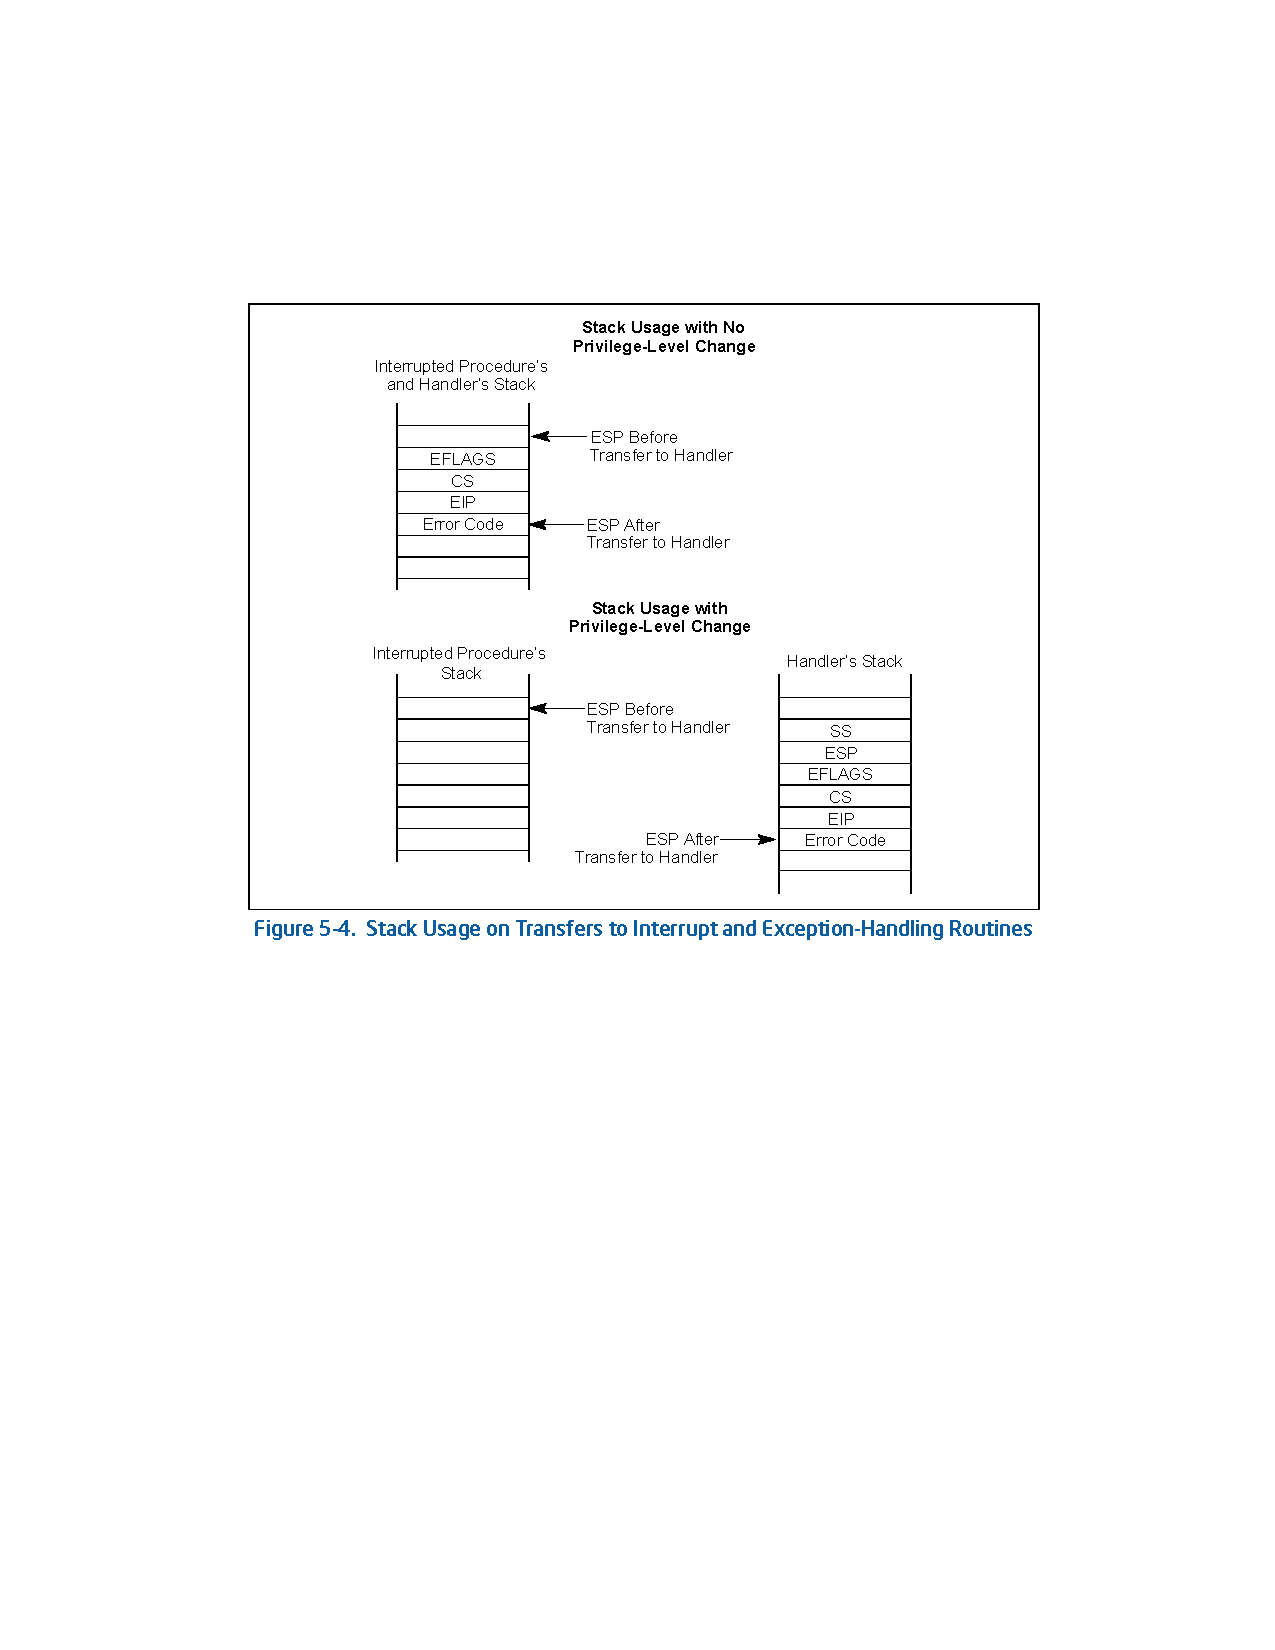
\includegraphics[scale=0.70]{img/stack.pdf}} \end{textblock} %
\end{frame}

\begin{frame}[fragile,t]
\frametitle{Scheduler: Cambio de nivel de privilegio}
    \begin{textblock}{100}(12,16) \only<1->{\includegraphics[scale=0.9]{img/stack_level0_leve3-layer1.pdf}} \end{textblock} %
    \begin{textblock}{100}(12,16) \only<2->{\includegraphics[scale=0.9]{img/stack_level0_leve3-layer2.pdf}} \end{textblock} %
    \begin{textblock}{100}(12,16) \only<3->{\includegraphics[scale=0.9]{img/stack_level0_leve3-layer3.pdf}} \end{textblock} %
    
    \begin{textblock}{100}(12,16) \only<4-4>{\includegraphics[scale=0.9]{img/stack_level0_leve3-layer4.pdf}} \end{textblock} % pr code 1
    \begin{textblock}{100}(12,16) \only<5->{\includegraphics[scale=0.9]{img/stack_level0_leve3-layer7.pdf}} \end{textblock} % line code 1
    \begin{textblock}{100}(12,16) \only<5-7>{\includegraphics[scale=0.9]{img/stack_level0_leve3-layer5.pdf}} \end{textblock} % pr code 2
    \begin{textblock}{100}(12,16) \only<5->{\includegraphics[scale=0.9]{img/stack_level0_leve3-layer13.pdf}} \end{textblock} % time 1
    \begin{textblock}{100}(12,16) \only<6->{\includegraphics[scale=0.9]{img/stack_level0_leve3-layer16.pdf}} \end{textblock} % cs ds 1
    \begin{textblock}{100}(12,16) \only<7->{\includegraphics[scale=0.9]{img/stack_level0_leve3-layer20.pdf}} \end{textblock} % pila n3
    
    \begin{textblock}{100}(12,16) \only<8->{\includegraphics[scale=0.9]{img/stack_level0_leve3-layer8.pdf}} \end{textblock} % line code 2
    \begin{textblock}{100}(12,16) \only<8-8>{\includegraphics[scale=0.9]{img/stack_level0_leve3-layer6.pdf}} \end{textblock} % pr code 3
    \begin{textblock}{100}(12,16) \only<8->{\includegraphics[scale=0.9]{img/stack_level0_leve3-layer19.pdf}} \end{textblock} % pila n0
    
    \begin{textblock}{100}(12,16) \only<9-9>{\includegraphics[scale=0.9]{img/stack_level0_leve3-layer10.pdf}} \end{textblock} % pr int 1
    \begin{textblock}{100}(12,16) \only<10->{\includegraphics[scale=0.9]{img/stack_level0_leve3-layer12.pdf}} \end{textblock} % line int    
    \begin{textblock}{100}(12,16) \only<10->{\includegraphics[scale=0.9]{img/stack_level0_leve3-layer14.pdf}} \end{textblock} % time 2
    \begin{textblock}{100}(12,16) \only<10->{\includegraphics[scale=0.9]{img/stack_level0_leve3-layer17.pdf}} \end{textblock} % cs ds 2
    \begin{textblock}{100}(12,16) \only<10-10>{\includegraphics[scale=0.9]{img/stack_level0_leve3-layer11.pdf}} \end{textblock} % pr int 2
    
    \begin{textblock}{100}(12,16) \only<11->{\includegraphics[scale=0.9]{img/stack_level0_leve3-layer21.pdf}} \end{textblock} % pila n3 arrow
    \begin{textblock}{100}(12,16) \only<11-11>{\includegraphics[scale=0.9]{img/stack_level0_leve3-layer6.pdf}} \end{textblock} % pr code 3
    
    \begin{textblock}{100}(12,16) \only<12->{\includegraphics[scale=0.9]{img/stack_level0_leve3-layer9.pdf}} \end{textblock} % line code 3
    \begin{textblock}{100}(12,16) \only<12->{\includegraphics[scale=0.9]{img/stack_level0_leve3-layer15.pdf}} \end{textblock} % time 3
    \begin{textblock}{100}(12,16) \only<12->{\includegraphics[scale=0.9]{img/stack_level0_leve3-layer18.pdf}} \end{textblock} % cs ds 3
\end{frame}

\begin{frame}
    \frametitle{Scheduler: Observaciones}
    \begin{textblock}{80}(0,20)
    \begin{itemize}
    \setlength\itemsep{0.5cm}
    \item[-]<2-> Siempre que hay un cambio de privilegio hay un cambio de pila.
    \item[-]<3-> Implica cambiar el \texttt{SS} y \texttt{ESP} por el correspondiente en su nivel de privilegio.
    \item[-]<4-> El resto de los segmentos de datos \texttt{DS}, $\cdots$, \texttt{ES} no se modifican.
    \end{itemize}
     \end{textblock}
    \begin{textblock}{100}(87,1) \includegraphics[scale=0.58]{img/TSS.pdf} \end{textblock}
\end{frame}

% \begin{frame}[plain]
% \Huge \textcolor{naranjauca}{Trabajo Práctico}
% \end{frame}
% 
% \begin{frame}[fragile]
% \frametitle{Game \textbf{Data} }
% \begin{figure}[ht!]
% 	\centering
% 	\includegraphics[scale=0.65]{../../tps/tp3/enunciado/img/game.pdf}
% \end{figure}
% \pause
% \begin{itemize}
% \footnotesize
%  \item[-] Posición de cada tarea: \texttt{PosTask[tasks]}
%  \item[-] Posición de cada portal: \texttt{PosPortal[tasks]}
%  \item[-] Tipo de cada tarea: \texttt{Type[tasks]}. (Rick-C137, Rick-D248, o Cronenberg).
%  \item[-] Tareas vivas: \texttt{Alive[tasks]}
%  \item[-] Contador de tareas vivas de cada Rick: \texttt{Count[player]}
%  \item[-] Tarea ejecutando actualmente: \texttt{current}
% \end{itemize}
% \end{frame}
% 
% \begin{frame}[fragile]
% \frametitle{Game \textbf{Syscalls} }
% \begin{itemize}
% \setlength\itemsep{0.4cm}
%  \item
%  \small \textcolor{naranjauca}{Syscall {\large \texttt{usePortalGun}} } int {\large \verb|137| }
% \begin{tabular}[h]{p{5.5cm}|p{7.5cm}}
% \small Parámetros  & Descripción \\
% \hline
% \verb| in EAX|$=$\verb|x|         & Desplazamiento en \verb|x| \\
% \verb| in EBX|$=$\verb|y|         & Desplazamiento en \verb|y| \\
% \verb| in ECX|$=$\verb|cross|     & \verb|0|: No cruzar, \verb|1|: Cruzar \\
% \verb| in EDX|$=$\verb|withMorty| & \verb|0|: Sin Morty, \verb|1|: Con Morty \\
% \hline
% \verb|out EAX|$=$\verb|worked|    & \verb|0|: No creado, \verb|1|: Creado\\
% \end{tabular}
% \item
% \small \textcolor{naranjauca}{Syscall {\large \texttt{IamRick}} } int {\large \verb|138| }
% \begin{tabular}[h]{p{5.5cm}|p{7.5cm}}
% \small Parámetros  & Descripción \\
% \hline
% \verb| in AX|$=$\verb|code|         & Código de identificación de universos. \\
%                                     & \verb|code|$=$\verb|0xC137| para Rick C-137 \\
%                                     & \verb|code|$=$\verb|0xD248| para Rick D-248 \\
% \end{tabular}
% \item
% \small \textcolor{naranjauca}{Syscall {\large \texttt{whereIsMorty}} } int {\large \verb|139| }
% \begin{tabular}[h]{p{5.5cm}|p{7.5cm}}
% \small Parámetros  & Descripción \\
% \hline
% \verb|out EAX|$=$\verb|x|         & Desplazamiento entre Rick y Morty en \verb|x| \\
% \verb|out EBX|$=$\verb|y|         & Desplazamiento entre Rick y Morty en \verb|y| \\
% \end{tabular}
% \end{itemize}
% \end{frame}
% 
% \begin{frame}[fragile]
% \frametitle{Game \textbf{Scheduler} }
%     \begin{textblock}{150}(12,12)
%     \includegraphics[scale=0.56]{../../tps/tp3/enunciado/img/sched_example.pdf}\\
%     \small Se debe tener un estado que indique cual es la tarea actual y cual debe ser la próxima tarea a ejecutar.
%     \end{textblock}
% \end{frame}
% 
% \begin{frame}[fragile]
% \frametitle{Game \textbf{Modo Debug} }
%     \begin{textblock}{100}(12,12) \only<1->{\includegraphics[scale=0.29]{img/figura_debug-layer1.pdf}} \end{textblock} %
%     \begin{textblock}{100}(12,12) \only<2->{\includegraphics[scale=0.29]{img/figura_debug-layer2.pdf}} \end{textblock} %
%     \begin{textblock}{100}(12,12) \only<3->{\includegraphics[scale=0.29]{img/figura_debug-layer3.pdf}} \end{textblock} %
%     \begin{textblock}{100}(12,12) \only<4->{\includegraphics[scale=0.29]{img/figura_debug-layer4.pdf}} \end{textblock} %
%     \begin{textblock}{70}(77,10)
%     \begin{enumerate}
%     \setlength\itemsep{1cm}
%      \item[-]<2-> Se presiona la tecla ``y'' y se activa/desactiva el modo debug.
%      \item[-]<3-> Alguna tarea produce una excepción, de estar en modo debug se detiene la ejecución mostrando la patalla de estado. El sistema continua funcionando, pero solo se ejecuta la tarea Idle.
%      \item[-]<4-> Cuando se presiona la tecla ``y'' nuevamente, se reanuda la ejecución.
%     \end{enumerate}
%     \end{textblock}
% \end{frame}
% 
% \begin{frame}[t,fragile]
% \frametitle{Ayudas}
% \begin{textblock}{100}(40,10)
% ASM para usar desde C (i386.h)
% \scriptsize
% \begin{verbatim}
% void lcr0(unsigned int val)  ; Escribir CR0
% unsigned int rcr0(void)      ; Leer CR0
% 
% void lcr1(unsigned int val)  ; Escribir CR1
% unsigned int rcr1(void)      ; Leer CR1
% 
% void lcr2(unsigned int val)  ; Escribir CR2
% unsigned int rcr2(void)      ; Leer CR2
% 
% void lcr3(unsigned int val)  ; Escribir CR3
% unsigned int rcr3(void)      ; Leer CR3
% 
% void lcr4(unsigned int val)  ; Escribir CR4
% unsigned int rcr4(void)      ; Leer CR4
% 
% void ltr(unsigned short sel) ; Escribir TR
% unsigned short rtr(void)     ; Leer TR
% 
% void tlbflush(void)          ; Flush de TLB
% 
% void breakpoint(void)        ; Generar un breakpoint
% \end{verbatim}
% \end{textblock}
% \end{frame}

\begin{frame}[fragile]
    \frametitle{Bibliografía: Fuentes y material adicional}
    \begin{itemize}
    \item Convenciones de llamados a función en x86: \\
    \url{https://en.wikipedia.org/wiki/X86_calling_conventions}
    \item Notas sobre System V ABI: \\
    \url{https://wiki.osdev.org/System_V_ABI}
    \item Documentación de NASM: \\
    \url{https://nasm.us/doc/}
    \item Artículo sobre el flag \texttt{-pie}: \\
    \url{https://eklitzke.org/position-independent-executables}
    \item Documentación de System V ABI: \\
    \url{https://uclibc.org/docs/psABI-x86_64.pdf}
    \item Manuales de Intel: \\
    \url{https://software.intel.com/en-us/articles/intel-sdm}
    \end{itemize}
\end{frame}

\begin{frame}[plain]
    \begin{center}
    \vspace{2cm}
    \huge ¡Gracias!\\
    \vspace{2cm}
    \normalsize Recuerden leer los comentarios al final de \\ este video por aclaraciones o fe de erratas.
    \end{center}
\end{frame}

\end{document}
